\documentclass[nocrop]{bioinfo}
\copyrightyear{2020} \pubyear{2020}

\usepackage{mathtools}
\usepackage{amsmath}
\usepackage{multirow}
\usepackage{graphicx}
\usepackage{tabularx}



\access{Advance Access Publication Date: 14/12/2020}
\appnotes{Scientific article}

\begin{document}
\firstpage{1}

\subtitle{Structural bioinformatics}

\title[LAB2 Project Rosaria Tornisiello]{GOR method vs Support Vector Machines for predicting protein secondary structure from amino-acid sequence}
\author[]{Rosaria Tornisiello\,$^{\text{\sfb 1,}*}$}
\address{$^{\text{\sf 1}}$Department of Pharmacy and Biotechnology, University of Bologna, Bologna,40126,Italy\\}

\corresp{$^\ast$To whom correspondence should be addressed.}

\abstract{\textbf{Motivation:} While the advent of large-scale sequencing techniques led to an exponential increase of protein sequence data, the experimental determination of protein structure is still in development. Being able to predict protein structure is the key issue for protein functional annotation. Therefore, several structure prediction methods have been developed over the last 70 years. Here we compare the performances of GOR method (Garnier-Osguthorpe-Robson) and Support Vector Machines (SVM) which are respectively based on Bayesian statistical analysis and machine learning.\\
\textbf{Results:} The results show how the machine learning based method performs slightly better than the GOR method, giving a more accurate prediction of the test set.\\
\textbf{Contact:} \href{name@bio.com}{rosaria.tornisiello@studio.unibo.it}\\
\textbf{Supplementary information:} Supplementary data are available at \textit{https://github.com/RosariaTornisiello/lb2-2020-project-Tornisiello}}

\maketitle
\section{Introduction}
Proteins are biopolymers composed of one or more aminoacidic chain. These macromolecules perform several functions such as catalysis, molecular recognition, structural support, intracellular transport and DNA replication, thanks also to their capacity to fold in multiple three-dimensional shapes. This suggests how knowing only the protein sequence is not sufficient to understand protein function. With the advent of next-generation sequencing techniques over 200 million protein sequences have been identified. Instead, given the high cost and the degree of difficulty of experimental protein structure determination, only about 170000 structures have been deposited \citep{yang2018sixty}. Although prediction of tertiary structure is one of the ultimate goals of protein science, the prediction of secondary structure from sequence is still a more feasible intermediate step in this direction. Moreover, knowledge about the secondary structure allows to adopt a divide and conquer approach to solve the full three-dimensional structure. This method is based on the prediction of simplified aspects of the structure, namely the key structural elements of the protein and the location of these elements not in the three-dimensional space but along the protein amino acid sequence. Consequently, the accuracy of protein secondary structure prediction directly impacts the accuracy of the overall protein structure determination \citep{yang2018sixty}. Moreover, secondary structure prediction plays a central role in the classification of unstructured and intrinsically disordered proteins.  
Secondary structure prediction method are classified in three categories: 
\begin{itemize}
\item First-generation methods: secondary structure was predicted based on the sequence according to the propensity of each amino acid residue to a specific secondary structure element. The representative method of this category is the Chou–Fasman method \citep{chou1974prediction}. 
\item Second-generation methods: used a sliding window of 3-51 neighbouring residues and statistical information. This class is represented by the GOR method that we will describe later \citep{garnier1978analysis}.
\item Third-generation: predicted secondary structure by using evolutionary information derived from multiple alignment of homologs sequences. The most popular predictor available of this generation is PSIPRED \citep{jones1999protein} which uses a two-stage neural network and is based on the position specific scoring matrices generated by PSI-BLAST. Other methods belonging to this group are: SSPro2 \citep{magnan2014sspro}, JPred4 \citep{drozdetskiy2015jpred4} and PHDsec/PROFsec \citep{rost1993improved}.
\end{itemize}
Accuracy improved with advancing generation firstly thanks to the inclusion of neighbouring residues within the window and secondly thanks to the usage of evolutionary information. 
In this project we compare second-generation and third-generation methods: GOR method and SVM. Both methods are trained on the JPred4 dataset \citep{drozdetskiy2015jpred4}, the trained model are validated by means of a 5-fold cross-validation (CV) and finally tested on a blind test set. The performances are evaluated according to Matthews correlation coefficient, precision, recall and accuracy. 
Our results show that SVM is able to predict the secondary structure conformation of our test set with an higher accuracy than the GOR method by 4\%, performing particularly better in the prediction of the Helix conformation.  
%%%%%%%%%%%%%%%%%%%%%%%%%%%%%%%%%%%%%%%%%%%%%%%%%%%%%%%%%%%%%%%%%%%%%%%%%%%%%%%%%%%%%%%%%%%%%%%%%%%
\begin{methods}
\section{Materials and Methods}
\subsection{Training dataset}
\subsubsection{General description}
The GOR model and the SVM were trained both on the same training dataset used for the JPred4 prediction method. This dataset was generated by selecting the representatives from SCOP \citep{fox2014chandonia} super-family level. Given that the SCOP classification is structure-based, this approach lessens the probability of including trivially detectable sequence similarities in the training dataset. The production of the JPred4 dataset started with 1987 representative sequences for each super-family in SCOPe v.2.04. Sequences are filtered and removed thereafter, according to the following criteria:
\begin{itemize}
\item structure resolution >2.5 Angstrom; 
\item sequences with length <30 residues since they are unlikely to represent globular protein domains;
\item sequences with length >800 residues due to the time required for building the sequence profiles;
\item multi-chain or fragment domains;
\item sequences with missing DSSP information for >9 consecutive residues;
\item inconsistencies between PDB, DSSP and other file definitions.
\end{itemize}
The described filtering process left a total of 1507 domain sequences. Afterwards, the obtained dataset was separated into two parts: a training set with 1357 sequences and a blind-test set composed by 150 sequences. In our work the blind-test set was generated in a separate pipeline. 

\subsubsection{Statistical analysis of JPred4 dataset}
In order to inspect the training set and check if it was a good representative of the protein space, we performed basic statistical analysis by means of a python pipeline developed in house, and compared the results with the UniprotKB/Swiss-Prot statistics as of October 2020.
We started analysing the taxonomic classification of the training set, shown as a pie plot in figure 1. 
\vspace{-15pt}
\begin{figure}[!tbh]%figure1
\centering
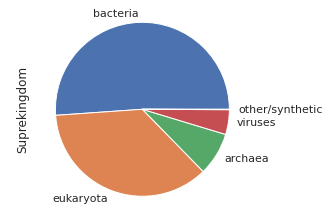
\includegraphics[width=6cm, height=4cm]{./plotsJPred4/Superkingdom.png}
\vspace{-15pt}
\caption{Pie plot that shows the taxonomic classification of the JPred4 dataset, obtained using the pandas package.}\label{fig:01}
\end{figure}
\vspace{-8pt}
Comparing our Super-kingdom distribution with the one shown in the SwissProt statistics, it is clear that the proportions are maintained. The only noticeable difference is the presence of synthetic proteins that were not removed from the JPred4 dataset.
The amino-acidic and the secondary structure composition of the training dataset are illustrated in the barplot in figure 2 and in the pieplot in figure 3, respectively. Both the distributions are comparable to the SwissProt ones, however, figure 3 shows an evident bias towards the helix composition due to the approximated grouping of secondary structure conformations described in section 2.2.2.
\begin{figure}[!tbh]%figure2
\centering
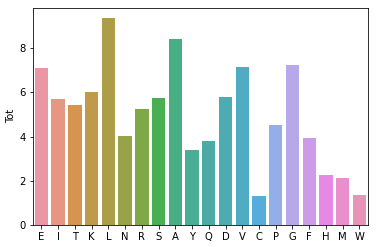
\includegraphics[width=7cm, height=4cm]{./plotsJPred4/aa_composition.png}
\vspace{-15pt}
\caption{Barplot that shows the amino-acidic composition of the JPred4 dataset, obtained using the seaborn package.}\label{fig:02}
\end{figure}

The barplot in figure 4 shows the propensity of each amino-residue type towards the three different secondary structure conformations. In particular the amino-acid types are ordered from left to right according to the physio-chemical properties: the first group is composed by apolar residues, followed by the aromatic group, the polar group and the charged group. This configuration allows to highlight the correlation between physio-chemical properties and secondary structure propensity of each residue type. The amino acids that tend to form $\alpha$-elix are: Ala, Leu, Glu, Gln, Arg, Met, Lys; instead, Val, Ile, Tyr, Phe, Thr and and Trp are prone to be in $\beta$-strands. Cys and His tend to be unstructured residues and all the remaining ones are likely to be found in the coil conformation. 
\begin{figure}[!tbh]%figure3
\centering
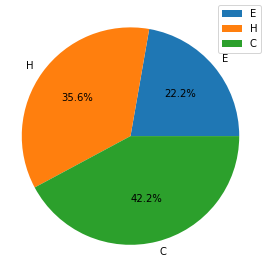
\includegraphics[width=4cm, height=4cm]{./plotsJPred4/ss_composition.png}
\vspace{-15pt}
\caption{Barplot that shows the secondary structure composition of the JPred4 dataset, obtained using the pandas package.}\label{fig:03}
\end{figure}
Alpha-helix admirers do not have polar heteroatoms on $C_{\beta}$ and $C_{\gamma}$ atoms, nor branching or aromatic group on $C_{\beta}$ atom. Amino acids that have aromatic groups or branching on $C_{\beta}$ atom are strand admirers. Turn and bend admirers have polar heteroatom on $C_{\beta}$ or $C_{\gamma}$ atoms or do not have $C_{\beta}$ atom at all \citep{malkov2005correlations}. These correlations seem to be approximately maintained in our dataset, as highlighted by figure 4 (considering turns and bends belonging to the coil class). 
%\vspace{-9pt}
As it is evident from the figure 5, the training set covers all the SCOP classes. Moreover, we generated a probability density distribution of the protein sequences length of this dataset that is available in the supplementary materials. Finally we can confirm the goodness of the JPred4 dataset, given its high similarity with the SwissProt database. 
%\vspace{-6pt}
\begin{figure*}[!h]%figure4
        \begin{minipage}{0.45\textwidth}
        \centering
        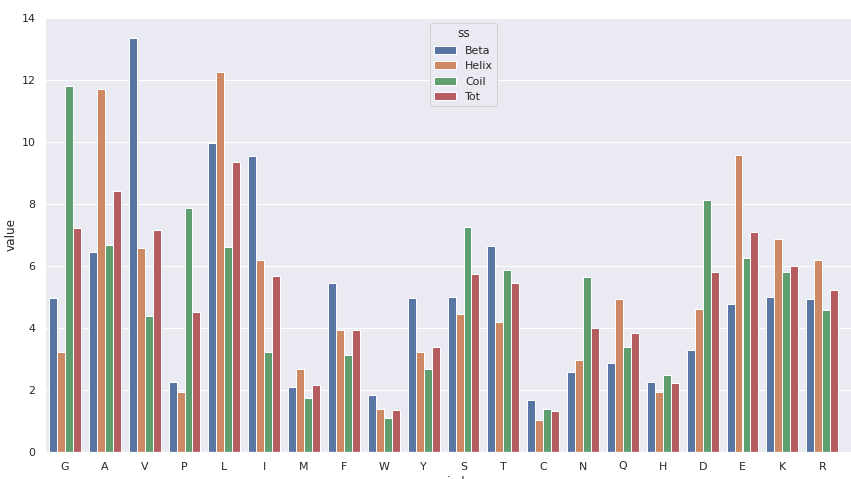
\includegraphics[width=8.5cm, height=5.5cm]{./plotsJPred4/aa_composition_per_ss.png}
        \vspace{-20pt}
        \caption{Barplot that shows the secondary structure distribution for each amino-acid type of the JPred4 dataset, obtained using the seaborn package.}\label{fig:04}
        \end{minipage}\hfill
        \begin{minipage}{0.45\textwidth}
        \vspace{+30pt}
        \centering
        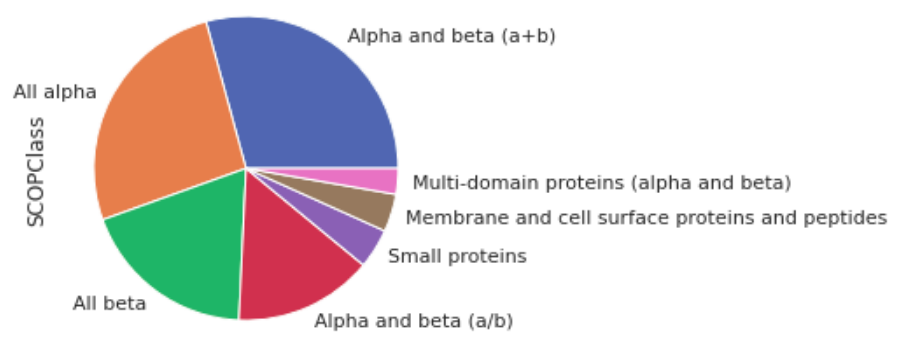
\includegraphics[width=8cm]{./plotsJPred4/SCOPClass.png}
        \vspace{+20pt}
        \caption{Pie plot that shows the relative abundance of each SCOP class in the training dataset, obtained using the pandas package.}\label{fig:05}
        \end{minipage}
\end{figure*}

\subsection{Blind-test dataset}
\subsubsection{Selection of 150 entries}
In order to evaluate the performance of both models, a separate blind-test set was generated, which is composed by samples totally independent from the training set so as to avoid prediction biases. First of all, we carried out an advanced search on RCSB PDB \citep{berman2000protein} setting the following filters:
\begin{itemize}
\item release date >= 01/01/2015;
\item experimental method: X-ray diffraction;
\item refinement resolution <= 2.5 Angstrom;
\item polymer entity sequence length between 50 and 300 residues;
\item polymer entity type: protein.
\end{itemize}
Applying these filters we ended up with 24714 PDB entries. Then we downloaded the PDB ids list and retrieved the correspondent fasta sequences. Implementing a python pipeline, we checked again the length of the single fasta chains and their composition, removing the ones with less then 50 and more that 300 residues length and the ones containing unidentified residues ("X" characters). In order to avoid over-representation of certain SCOP classes, we lowered the internal redundancy below 30\% by clustering the remaining chains using MMseqs2 (Many-against-Many sequence searching) which is a software suite to search and cluster huge protein and nucleotide sequence sets \citep{steinegger2017mmseqs2}. The chosen clustering criteria were: minimum sequence identity of  30\%, length coverage threshold equals to 0.5 and an e-value threshold of 0.001. Following these steps we obtained 4760 representative protein entities. The last filtering step was the removal of the external redundancy through BLASTp \citep{altschul1990basic}. Firstly, the JPred4 dataset was formatted as database with the \textit{makeblastdb} tool, then all the cluster representatives were compared to it setting an e-value threshold of 0.01, finally all entries with a sequence identity equals or higher than 30\% were excluded. In order to build the final blind-test set, 150 random sequences were selected from the remaining ones and their matching PDB files were downloaded.

\subsubsection{Retrieving the secondary structure}
By means of an in-house developed bash pipeline, we further skimmed the structure files obtained in the previous steps, selecting only the protein chains of interest. The following procedure was the usage of the DSSP program \citep{kabsch1983dictionary} to derive the secondary structure of the selected chains. The DSSP program defines secondary structure, geometrical features and solvent exposure of proteins, given atomic coordinates in Protein Data Bank format (PDB) or macro-molecular Crystallographic Information File format (mmCIF). DSSP is able to assign the following 8 different secondary structure conformations: $\alpha$-helix (H), $\beta$-bridge residue (B), extended strand (E), 3/10-helix (G), 5-helix (I), H-bonded turn (T), bend (S) or empty. In order to simplify the classification, in our work we grouped them as:
\begin{itemize}
    \item H, G and I classified as H;
    \item B and E classified as E;
    \item T, S and empty classified as C or "-".
\end{itemize}
Once obtained the DSSP output files, both the secondary structure sequence and the primary sequence were extracted in FASTA format by means of an in-house developed python script.
\subsubsection{Statistical analysis of the blind-test set}
As for the training dataset, some basic statistical analysis have been performed to inspect the sequence length, the amino-acidic composition and the secondary structure conformation distribution of the test set. The resulting plots are available in the supplementary materials. It is possible to confirm that our test set has been generated in compliance with the JPred4 dataset and with the protein space properties.
\subsection{Sequence profiles generation}
As previously said, new generation methods for predicting secondary structure avail of evolutionary information to improve the prediction performance. In particular they are based on the use of sequence profiles obtained from multiple sequence alignments (MSA). Since sequence profiles summarize the MSA from which they are derived, gathering information about protein families including also distantly related homologs, they enable the predictor to reach a much higher accuracy than the simple prediction of the first-generation methods. 
In our work, in order to obtain the sequence profiles of both the training and test set, we searched all the sequences belonging to them in a large sequence database obtained indexing the UniprotKB/SwissProt database \citep{uniprot2019uniprot} using the \textit{makeblastdb} tool. Then the PSI-BLAST (Position-Specific Iterative BLAST, \citep{altschul1997gapped}) algorithm was used to search for homologs sequences in the obtained database. The procedure PSI-BLAST uses can be summarized in five steps:
\begin{enumerate}
    \item PSI-BLAST takes as an input a single protein sequence and compares it to a protein database, using the gapped BLAST program.
    \item The program constructs a multiple alignment, and then a profile, from any significant local alignments found.
    \item The program compares the profile to the protein database, again seeking local alignments. After a few minor modifications, the BLAST algorithm can be used for this directly.
    \item PSI-BLAST estimates the statistical significance of the local alignments found.
    \item Finally, PSI-BLAST iterates, by returning to step (2), an arbitrary number of times or until convergence.
\end{enumerate}
PSI-BLAST uncovers many protein relationships missed by single-pass database-search methods. In our case PSI-BLAST was executed setting an e-value threshold equal to 0.01, maximum number of iterations equal to 3 and number of descriptions equal to 10000. This program returns as output for each sequence given as input, the Position-Specific Substitution Matrix (PSSM) computed during the search and the file containing the pairwise alignments. In order to extract the sequence profiles, the PSSM files are then parsed through a python script developed in house. Finally, for both the training and the blind-test set the sequence profiles were parsed removing all the 0 matrices arose due to PSI-BLAST not finding any similarity in the database. At the end of the described procedure, we obtained 1204 training profiles and 117 test profiles. 

\subsection{The GOR method}
\subsubsection{General overview}
The GOR program is one of the first major methods proposed for protein secondary structure prediction from sequence. The original article (GOR I) was published by Garnier, Osguthorpe, and Robson in 1978, however, the method has been continuously improved and modified for 30 years with the last GOR V version published in 2002. The GOR algorithm was modified to include the triplet statistics within the window. The previous versions of the program used only single residue statistics (GOR I–II) or the combination of the single residue and pair residue statistics within the window (GOR III–IV). The most important improvement was the inclusion of multiple sequence alignments from PSI-BLAST program, which allows to take into account evolutionary information for the secondary structure prediction \citep{kloczkowski2002combining}.
The GOR algorithm is based on information theory combined with Bayesian statistics. One of the basic mathematical tools of information theory is the information function I(S,R):
\begin{equation}\label{eq:01}
    I(S; R) = \log \frac{P(S|R)}{P(S)} = \log \frac{P(S, R)}{P(R)P(S)}
\end{equation}
For the problem of protein secondary structure prediction, the information function is defined as the logarithm of the ratio of the conditional probability P(S|R) of observing conformation S, (where S is one of the three states: helix (H), extended (E), or coil (C)) for residue R (where R is one of the 20 possible amino acids) and the probability P(S) of the occurrence of conformation S. The conformational state of a given residue in the sequence depends not only on the type of the amino acid R but also on the neighboring residues along the chain within the sliding window. GOR IV used a window of 17 residues, that is, for a given residue, eight nearest neighboring residues on each side were analyzed. According to information theory, the information function defined over the window of residues centered at a given residue position $R_0$, considering d equal to 8, is expressed as:
\begin{equation}\label{eq:02}
\begin{split}
    I(S; R_{-d},\dots,R_{d}) =& \log \frac{P(S|R_{-d},\dots,R_d)}{P(S)} =\\
    &\log \frac{P(S,R_{-d},\dots,R_d)}{P(R_{-d},\dots,R_d)P(S)}
\end{split}
\end{equation}
Computing all the joint probabilities of S and all the possible residues in all the positions of the window is computationally expensive since we would have an exponential number of possible configurations. Moreover, we would need a very large sequence database to estimate reliable distributions. The solution of this problem is to assume statistical independence of all the 17 residues within the window. Given this statement, the previous formula can be expressed as:
\begin{equation} \label{eq:03}
    I(S; R_{-d},\dots,R_{d})\approx \sum_{k=-d}^{d}I(S; R_{k})
\end{equation}
The window-based information function is equal to the sum of the single residue functions. The parameters needed to compute the equation (\ref{eq:03}) are:
\begin{itemize}
    \item $P(R_k,S)$: probability of observing a residue of type R at position k in the window and the central residue $R_0$ in conformation S:
    \item $P(R_k)$: probability of observing a residue of type R at position k in the window;
    \item $P(S)$: probability of observing conformation S.
\end{itemize}
The GOR method training phase consists in the computation of a matrix containing the information function for each position in the sliding window, considering all kinds of secondary structure conformation and residue. The information matrix is then used to predict the secondary structure of a test set of protein sequences, given their profiles. During the prediction phase, each residue position of all the query sequences is analyzed, associating it with the conformation S characterized by the highest value in the information matrix, that is:
\begin{equation}
    S = \arg\max_{S}\sum_{k=-d}^{d}I(S; R_{k})
\end{equation}
\subsubsection{Implementation}
In this project we implemented the GOR model by means of two python pipelines developed in-house. The first python script is dedicated to the training of the model, that is the generation of the information function. It takes as input the training set UniProt IDs list, the training set sequence profiles (in which we inserted the secondary structure sequence defined by DSSP), and gives as output the information matrix. The latter is given as input to the prediction python script, along with the test set UniProt IDs list and their sequence profiles. The final outputs of our GOR method implementation are the predicted secondary structure sequences of all the test set entries, stored in FASTA files. 

\subsection{Support Vector Machines} 
\subsubsection{General description and geometrical interpretation}
A Support Vector Machine (SVM) is a supervised machine learning approach that is able to perform both classification and regression analysis. For the purpose of this project, we will focus on the Support Vector Classifiers (SVC).  The goal of a SVC is to separate two classes of data using a function which is induced from the training examples. The final classifier must be able to generalize unseen data. 
\begin{figure}[!tbh]%figure6
\centering
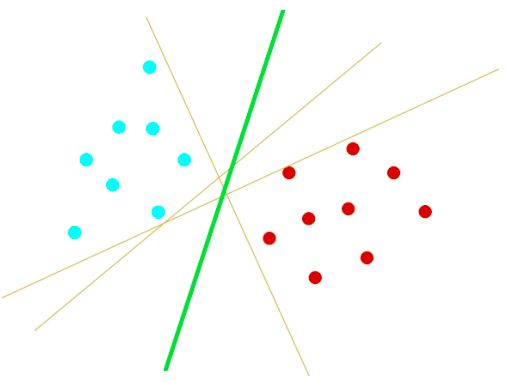
\includegraphics[scale=0.25]{./plotsJPred4/SVM_1.png}
\vspace{-15pt}
\caption{Optimal separating hyperplane \citep{gunn1998support}.}\label{fig:06}
\end{figure}

Considering the example in figure 6, we can see that it is possible to draw several separating linear classifiers, however, only one of them maximizes the distance between itself and the nearest points of each class: this classifier is defined as the optimal separating hyperplane. The latter is defined as the set of points $\Vec{x}$ characterized by the same projection on a given vector $\Vec{w}$:
\begin{equation}
    \Vec{w} \Vec{x}+b=0
\end{equation}
A separating hyperplane in canonical form must satisfy the following constraints:
\begin{equation}
    y^i[\langle w, x^i \rangle  + b] \geq 1,  i = 1,\dots,l.
\end{equation}
The distance $d(w,b;x)$ of a point $x$ from the hyperplane $(w, b)$ is:
\begin{equation}
    d(w,b;x) = \frac{|\langle w, x^i \rangle + b|}{\|w\|}
\end{equation}
The optimal separating hyperplane will be the linear classifier that maximizes the margin $\rho$, that is the one that minimizes $\|w\|$. It is possible to demonstrate that $\rho$ is equal to $\frac{2}{\|w\|}$; hence the hyperplane that optimally separates the data is the one that minimises:
\begin{equation}
    \Phi(w)= \frac{1}{2} \|w\|^2
\end{equation}
The solution to the optimisation problem of Equation 8 under the constraints of Equation 6 is given by the saddle point of the Lagrangian:
\begin{equation}
    L(\vec{w},b,\alpha_i) = \frac{1}{2}\|w\|^2 + \sum_i \alpha_i [1-y^i(\langle w, x^i \rangle+b)]
\end{equation}
The minimization of the Lagrangian (concave function) can be converted in the maximization of the Dual Lagrangian (convex function):
\begin{equation}
    \begin{split}
        &\bar{L}(\alpha_i) = -\frac{1}{2}\sum_i \sum_j \alpha_i \alpha_j y^i y^j x^i x^j + \sum_i \alpha_i \\
		&\alpha_i [1-y^j(\langle w, x^i \rangle+b)]=0 \ \forall \ i  \\
		&\alpha_i \geq 0 \ \forall \ i
    \end{split}
\end{equation}
SVC as described above is defined as \textit{hard margins SVC} since no margin violation is allowed. However, frequently, a \textit{soft margins SVC} is preferred because it produces a real valued output between ${-1}$ and $1$ when the classifier is queried within the margin, where no training data resides \citep{gunn1998support}. In this case we introduce the \textit{slack variable} $\xi_i$ to allow some misclassification:
\begin{equation}
\begin{split}
    minimize\ \ \ &\Phi(w,\xi)=\frac{1}{2}\|w\|^2 + C \sum_i \xi_i \\
    constrained\ \ by\ \ \ & y^i[\langle w, x^i \rangle  + b] \geq 1 - \xi_i \ \ \ \ \  \xi_i \geq 0, \forall i
\end{split}
\end{equation}
Where C is an hyperparameter that represents a trade-off between the minimization of $\xi$ and the maximization of $\rho$. 
When data are not linearly separable, we can apply the \textit{kernel trick}:  the idea is mapping the non-linearly separable dataset into a higher dimensional space where we can find an hyperplane that can separate the samples. As it is possible to observe in the Equation 10, the vector $\vec{x}$ appears only in the scalar product, consequently we can deduce that the optimization problem depends only on it. Hence, we can apply the kernel trick without explicitly computing the coordinates of the transformed data points. If we use a mapping function that maps our data into a higher dimensional space, then, the maximization will depend on the scalar products $\phi(\vec{x})\phi(\vec{y})$ of the mapping function for different samples. This scalar product is also defined as kernel function $K(\vec{x}, \vec{y})$.
The SVC implemented for this project uses the radial basis function (rbf) kernel that is formulated as follows:
\begin{equation}
		K(\vec{x},\vec{y}) = e^{(-\gamma\|\vec{x}-\vec{y}\|^2)}
\end{equation}
Where $\gamma$ is an hyperparameter.  
\subsubsection{Application of SVM for secondary structure prediction}
The problem of secondary structure prediction has been addressed by means of several machine learning models including multi-layer perceptrons, recurrent neural networks and SVMs which have proven to be promising classifiers. Indeed, SVMs are successful in controlling the classifier's potential for overfitting ensuring the maximization of $\rho$ \citep{ward2003secondary}. Other convenient aspects of SVMs are the use of few hyperparameters and the interchangeable use of kernel functions. Nevertheless, SVMs are not designed to perform multi-class classification analysis as the task at hand, but only binary ones. This issue is faced applying either the One-vs-Rest (OvR) or the One-vs-One (OvO) strategy: in the first case the multi-class classification is split into one binary classification problem per class, in the second case the multi-class classification is split into one binary classification problem per each pair of classes. Hence, the application of SVM for multiclass prediction using the OvR strategy consists in training $N$ binary SCV, where N is the number of classes,  or (N(N-1))/2 binary SVC adopting the OvO option. In our work, we chose to train the SVC using the OvR approach.

\subsubsection{Grid search}
Grid search is a process of hyperparameter optimization, i.e. the exploration of all the hyperparameter combinations to find the ones that yields the best machine learning predictor. In our work we performed a grid search analysis testing a C parameter equal to 2 or 4 and a $\gamma$ equal to 0.5 and 2. In principle, the grid search should explore also the kernel functions space, however, in our project we chose to maintain the default kernel function of the sklearn SVC (rbf) due to time constraints and limited computational power. 

\subsubsection{Implementation}
For the purpose of this project, training and testing of the SVC were both implemented using the scikit-learn (sklearn) python module, version 0.24 \citep{pedregosa2011scikit}, that is based on the LIBSVM library  \citep{chang2011libsvm}. The sklearn implementation allows to tune both the hyperparameters C and $\gamma$ and to set the desired kernel function. 
As regards the training phase, we started producing our SVC inputs i.e. the matrix of features and the array containing the classes of each sample of the training dataset. Each sequence profile, obtained as described in section 2.3, was parsed by means of a sliding window; each window was flattened and finally, all the windows were concatenated to generate the final matrix of features. Moreover, the secondary structure conformation defined by DSSP of each residue position was stored in an array, modifying the class attributes as follows: class 1 for Helix, class 2 for Strand and class 3 for Coil. Thereafter, we performed the fitting of our SVC. 
The prediction phase was then carried out, handling the test dataset with the very same procedure adopted for the training dataset. 

\subsection{Evaluation procedure and scoring measure}
\subsubsection{Scoring indexes}
In order to evaluate and compare the performances of both predictors we computed the following scoring indexes:
\begin{itemize}
\item Q3 score, the multiclass accuracy which  gives the percentage of amino acids for which the secondary structure conformation was correctly predicted \citep{spencer2014deep}. Considering two classes $i$ and $j$ with $1 < i,j < k$, we can compute the Q3 score as:
\begin{equation}
Q_3  = \frac{p_{11}+p_{22}+\dots+p_{kk}}{N}
\end{equation}
where $p_{i,j}$ is an object of class i predicted in class j and $N$ is the number of classes.

\item The Matthews correlation coefficient (MCC) that is a more reliable statistical rate which accounts for all of the four categories true positives (FP), false negatives (FN), true negatives (TN), and false positives (FP). When the classifier is perfect (FP = FN = 0) the value of MCC is 1, indicating perfect positive correlation. Conversely, when the classifier always misclassifies (TP = TN = 0), we get a value of -1, representing perfect negative correlation. In contrast with the accuracy, this rate is not affected by class imbalance. It is computed as:
\begin{equation}
    \text{MCC} = \frac{TP \times TN - FP \times FN}{\sqrt{(TP+FP)(TP+FN)(TN+FP)(TN+FN)}}
\end{equation}

\item Precision, also called positive predicted value, is the fraction of true positive over all the positive predictions. It is equal to:
\begin{equation}
    \text{Precision} = \frac{TP}{TP+FP}
\end{equation}

\item Recall, also called sensitivity, that is the proportion of actual positives correctly identified:
\begin{equation}
    \text{Recall} = \frac{TP}{TP+FN}
\end{equation}
\end{itemize}
The cross validation results are reported along with the mean and standard error that is computed as:
\begin{equation}
	\text{Standard error} = \frac{\sigma}{\sqrt{n}}
\end{equation}
Where $\sigma$ is the standard deviation and n is the number of samples, that in our case is equal to 5.
\subsubsection{Cross-validation} 
CV is a machine learning technique used to assess how accurately the model will predict a previously unseen dataset. The CV methods can be classified in two sub-categories:
\begin{itemize}
    \item Exhaustive CV: learn and test the model on all possible ways to divide the original sample into a training and a validation set;
    \item Non-exhaustive CV: do not compute all the possible ways of splitting the original sample.
\end{itemize}
In this project we performed a non-exhaustive, k-fold CV, by which the entire training set is partitioned in k equal sized subsets. Each subset is used as validation set to test the model by rotation, while the other $k-1$ subsets serve as training dataset. At the end of the process, the $k$ results are averaged to produce a single evaluation.

\end{methods}
%%%%%%%%%%%%%%%%%%%%%%%%%%%%%%%%%%%%%%%%%%%%%%%%%%%%%%%%%%%%%%%%%%%%%%%%%%%%%%%%%%%%%%%%%%%%%%%%%%%%%
\section{Results}
\subsection{Cross-validation results}
The 5-fold CV of both methods has been evaluated by means of the MCC computation. Table 1 lists the MCC scores computed for each fold of the GOR CV. While Table 2 stores the MCC scores for each fold of the 4 different SVC tested by means of grid search. For both methods, the mean is reported along with the standard error. 

\begin{table}[!tbh]
\centering
\resizebox{.45\textwidth}{!}{% 
\begin{tabular}{ c|c|c|c|c|c|c }
\toprule & fold 0 &  fold 1 &  fold 2 & fold 3 & fold 4 & Mean\\
\midrule
 MCC & 0.460 & 0.466  & 0.468  & 0.454 & 0.457 & 0.461 $\pm$ 0.002\\
\botrule
\end{tabular}}
\vspace{+10pt}
\caption{5-fold cross-validation MCC values, mean and standard error of GOR model.}
\label{Tab:01}
\end{table}

%\vspace{-15pt}
\begin{table}[!tbh]
\centering
\resizebox{.5\textwidth}{!}{% 
\begin{tabular}{ c| c| c| c| c }
\toprule
\multirow{2}{*}{Fold}  & $C=2$ & $C=2$ & $C=4$ & $C=4$\\
& $\gamma=0.5$ & $\gamma=2$ & $\gamma=0.5$ & $\gamma=2$\\
\midrule
 0 & 0.549 & 0.168 & 0.538 & 0.166\\
 1 & 0.552 & 0.185 & 0.544 & 0.181\\
 2 & 0.560 & 0.184 & 0.549 & 0.181\\
 3 & 0.538 & 0.168 & 0.529 & 0.166\\
 4 & 0.540 & 0.153 & 0.530 & 0.150\\
 \midrule
Mean & 0.548$\pm$0.003 & 0.171$\pm$0.004 & 0.538$\pm$0.003 & 0.169$\pm$0.004 \\\botrule
\end{tabular}}
\vspace{+10pt}
\caption{5-fold cross-validation MCC values, mean and standard errors for each SVC tested by means of grid search.}
\label{Tab:02}
\end{table}

As for the GOR method, the CV yielded a mean MCC of $0.461$ and a standard error of $0.002$. The 5 scores show no significant difference and a very low standard error meaning that the performance of the model for each fold is approximately equivalent. The slight difference between the MCC values is not surprising, given the subtle discrepancy in amino-acid composition and secondary structure distribution between the 5 subsets. 
The SVM CV was performed for each combination of the C and $\gamma$ parameters. The classifier that yielded the maximum MCC value was the one characterized by $C=2$ and $\gamma=0.5$, with a mean MCC equal to $0.548$ and a very low standard error of $0.003$. 

\subsection{Blind test results}  
Table 3 lists all the scoring indexes values for each secondary structure conformation of both models, obtained by the prediction phase of the blind test set. The MCC values are higher for the H conformation in both cases. However, it is possible to notice that the GOR model precision is higher for the C conformation, while the SVM is more precise in predicting the H conformation. Instead, concerning the recall, we have the inverse situation. The SVM prediction shows an overall three classes accuracy, Q3, higher than the GOR model.

\begin{table}[!tbh]
    \centering
    \resizebox{.35\textwidth}{!}{% 
    \begin{tabular*}{0.75\linewidth}{@{\extracolsep{\fill} }  c | c | c | r  }
    \toprule
    SCORE & SS & GOR & SVM\\
    \midrule
    \multirow{3}{*}{MCC} & H & 0.515 & 0.637\\
    & E & 0.466 & 0.517\\
    & C & 0.426 & 0.473\\
    \midrule
    \multirow{3}{*}{Precision} & H & 0.654 & 0.857\\
    & E & 0.551 & 0.813\\
    & C & 0.744 & 0.566\\
    \midrule
    \multirow{3}{*}{Recall} & H & 0.787 & 0.669\\
    & E & 0.683 & 0.444\\
    & C & 0.464 & 0.872\\
    \midrule
    Q3 & total & 0.643 & 0.687\\
    \botrule
    \end{tabular*}}
    \vspace{+10pt}
    \caption{Blind-test set scores for both the GOR and the SVM models, reported for each secondary structure conformation.}
    \label{Tab:03}
\end{table}

\subsection{Discussion of results} 
Firstly, we can observe that there is not a substantial difference in the MCC values between CV and test phase, meaning that both models can be considered good estimators since they are capable of generalize well the test set. 
The test phase evinced how the SVM is able to predict secondary structure conformation better than the GOR model with a 4\% disparity for the Q3 score.
This is a foreseeable outcome given that the GOR method is based on the assumption of statistical independence of all the 17 window residues while the SVM, thanks to its ability to handle large dataset, accounts for the correlations between neighbouring residues. Moreover, the GOR method performance could increase including all the GOR V improvements such as the the introduction of the decision constants in the final prediction of the conformational state, the inclusion of residues pairs and triplets and a smaller window of 13 residues \citep{sen2005gor}. Another important limitation imposed on both models implemented in this project is the bypassing of essential biological properties. Indeed, we arbitrarily defined only 3 states but ideal helices and sheets do not exist and there is not a precise boundary between the various conformations. Moreover, the described methods do not consider that helices involve hydrogen bonds of at least 4 neighbouring residues while sheets forms also thanks to hydrogen bonds between distant residues. Hence, another source of error could be the incapacity of these secondary structure prediction methods in considering non-local interactions: the important inter-sequence interactions are short ranged and only one-fourth of the total information needed to determine the secondary structure is available from local inter-sequence correlations \citep{crooks2004protein}.
\section{Conclusion}
The GOR model and the SVM proved to be both relatively good predictors, giving about $64\%$ and $69\%$ of Q3 score respectively. However, the higher performance of SVM is highly linked to an increase of the time complexity. While the training phase of the GOR model took a couple of seconds, the SVM one was a matter of days. State-of-the-art secondary structure prediction methods have reached an accuracy of about 84\% by means of powerful machine learning and deep learning techniques, however the theoretical accuracy limit of 88\% \citep{rost2001protein} could be obtained by capturing non-local interactions between residues that are close in the 3D space but far away in the primary structure. 
%%%%%%%%%%%%%%%%%%%%%%%%%%%%%%%%%%%%%%%%%%%%%%%%%%%%%%%%%%%%%%%%%%%%%%%%%%%%%%%%%%%%%%%%%%%%%%%%%%%%%%
\bibliographystyle{natbib}
\bibliography{reference.bib}

\begin{supplementary}
\section{Supplementary material}
\vspace{-35pt}
\begin{figure}[!h]
    \centering
    \begin{minipage}{0.5\textwidth}
    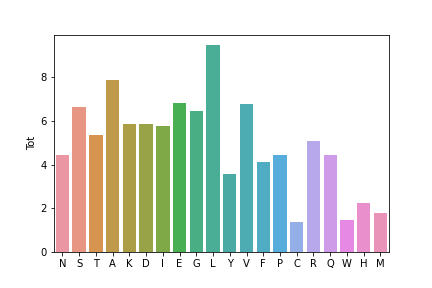
\includegraphics[scale=0.45]{./plotsJPred4/aa_composition_blind.png}
    \caption{Bar plot that shows the amino-acidic composition of the blind test dataset, obtained using the pandas package.}
    \end{minipage}\hfill
    \begin{minipage}{0.5\textwidth}
    \centering
    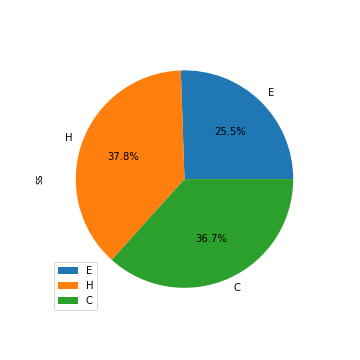
\includegraphics[scale=0.45]{./plotsJPred4/ss_composition_blind.png}
    \caption{Pie plot that shows the percentage of secondary structure conformations of the blind test dataset, obtained using the pandas package.}
    \end{minipage}
\end{figure}
\vspace{-20pt}
\begin{figure}[!h]
\centering
\captionsetup{}
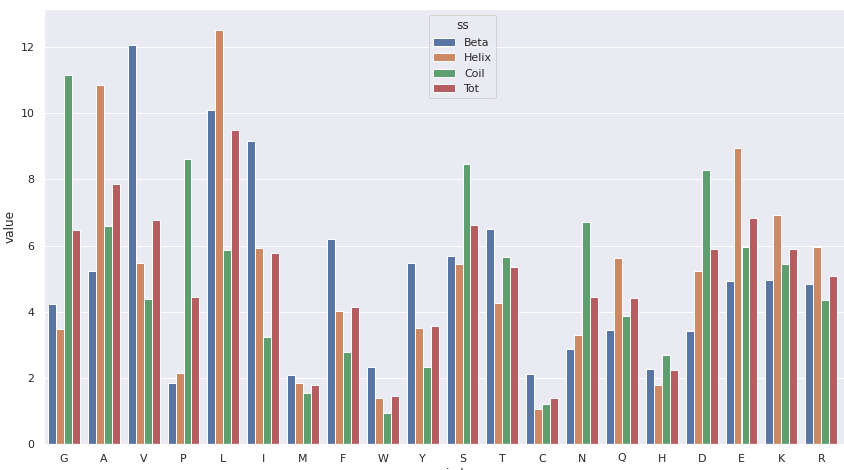
\includegraphics[scale=0.35]{./plotsJPred4/ss_per_aa_composition_blind.png}
\caption{Bar plot that shows the percentage of secondary structure conformations for each amino acid type of the blind test dataset, obtained using the seaborn package.}
\end{figure}

\begin{figure}[!h]
    \centering
    \begin{minipage}{0.45\textwidth}
    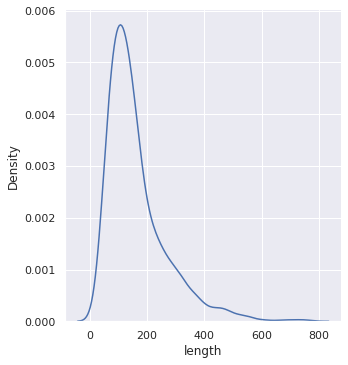
\includegraphics[scale=0.5]{./plotsJPred4/length_training.png}
    \caption{Probability density distribution of the sequences length of the training dataset, obtained using the seaborn package.}
    \end{minipage}\hfill
    \begin{minipage}{0.45\textwidth}
    \centering
    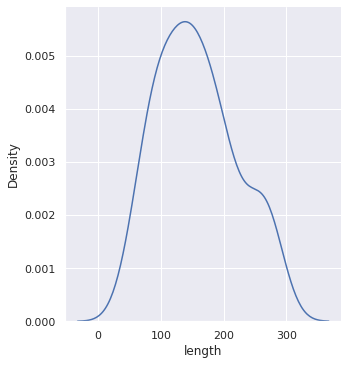
\includegraphics[scale=0.5]{./plotsJPred4/length_blind.png}
    \caption{Probability density distribution of the sequences length of the test dataset, obtained using the seaborn package.}
    \end{minipage}
\end{figure}

\end{supplementary}

\end{document}